\documentclass[11pt,]{article}
\usepackage{lmodern}
\usepackage{amssymb,amsmath}
\usepackage{ifxetex,ifluatex}
\usepackage{fixltx2e} % provides \textsubscript
\ifnum 0\ifxetex 1\fi\ifluatex 1\fi=0 % if pdftex
  \usepackage[T1]{fontenc}
  \usepackage[utf8]{inputenc}
\else % if luatex or xelatex
  \ifxetex
    \usepackage{mathspec}
  \else
    \usepackage{fontspec}
  \fi
  \defaultfontfeatures{Ligatures=TeX,Scale=MatchLowercase}
\fi
% use upquote if available, for straight quotes in verbatim environments
\IfFileExists{upquote.sty}{\usepackage{upquote}}{}
% use microtype if available
\IfFileExists{microtype.sty}{%
\usepackage{microtype}
\UseMicrotypeSet[protrusion]{basicmath} % disable protrusion for tt fonts
}{}
\usepackage[margin=1in]{geometry}
\usepackage{hyperref}
\hypersetup{unicode=true,
            pdftitle={Etude des effets des pésticides dans la production des vins de table},
            pdfauthor={Arnaud Blanc, Nikita Gusarov, Sasha Picon},
            pdfborder={0 0 0},
            breaklinks=true}
\urlstyle{same}  % don't use monospace font for urls
\usepackage{longtable,booktabs}
\usepackage{graphicx,grffile}
\makeatletter
\def\maxwidth{\ifdim\Gin@nat@width>\linewidth\linewidth\else\Gin@nat@width\fi}
\def\maxheight{\ifdim\Gin@nat@height>\textheight\textheight\else\Gin@nat@height\fi}
\makeatother
% Scale images if necessary, so that they will not overflow the page
% margins by default, and it is still possible to overwrite the defaults
% using explicit options in \includegraphics[width, height, ...]{}
\setkeys{Gin}{width=\maxwidth,height=\maxheight,keepaspectratio}
\IfFileExists{parskip.sty}{%
\usepackage{parskip}
}{% else
\setlength{\parindent}{0pt}
\setlength{\parskip}{6pt plus 2pt minus 1pt}
}
\setlength{\emergencystretch}{3em}  % prevent overfull lines
\providecommand{\tightlist}{%
  \setlength{\itemsep}{0pt}\setlength{\parskip}{0pt}}
\setcounter{secnumdepth}{0}
% Redefines (sub)paragraphs to behave more like sections
\ifx\paragraph\undefined\else
\let\oldparagraph\paragraph
\renewcommand{\paragraph}[1]{\oldparagraph{#1}\mbox{}}
\fi
\ifx\subparagraph\undefined\else
\let\oldsubparagraph\subparagraph
\renewcommand{\subparagraph}[1]{\oldsubparagraph{#1}\mbox{}}
\fi

%%% Use protect on footnotes to avoid problems with footnotes in titles
\let\rmarkdownfootnote\footnote%
\def\footnote{\protect\rmarkdownfootnote}

%%% Change title format to be more compact
\usepackage{titling}

% Create subtitle command for use in maketitle
\providecommand{\subtitle}[1]{
  \posttitle{
    \begin{center}\large#1\end{center}
    }
}

\setlength{\droptitle}{-2em}

  \title{Etude des effets des pésticides dans la production des vins de table}
    \pretitle{\vspace{\droptitle}\centering\huge}
  \posttitle{\par}
  \subtitle{Analyse empirique des marchés}
  \author{Arnaud Blanc, Nikita Gusarov, Sasha Picon}
    \preauthor{\centering\large\emph}
  \postauthor{\par}
      \predate{\centering\large\emph}
  \postdate{\par}
    \date{25/12/2019}

\usepackage{setspace}

% to make the first rows bold in tables
\usepackage{longtable}
\usepackage{tabu}
\usepackage{booktabs}

% Floats
\usepackage{morefloats}
\usepackage{float}
\usepackage{placeins}

% highlighting
\usepackage{soul}

% Short toc
\usepackage{shorttoc}
\setcounter{tocdepth}{1}

% referencing mutliple things with a single command - \cref
\usepackage{cleveref}

% Change section names style
\usepackage[dvipsnames]{xcolor}
% \usepackage{sectsty}

% \sectionfont{\color{Green}}  % sets colour of sections
% \subsectionfont{\color{Green}}  % sets colour of sub
% \subsubsectionfont{\color{Green}}  % sets colour of subsub

% this makes dots in table of contents
% \renewcommand{\cftsecleader}{\cftdotfill{\cftdotsep}}
% to change the title of contents
% \renewcommand{\contentsname}{Whatever}

% line numbers for review purposes
% this package might not be available in default latex installation 
% get it by 'sudo tlmgr install lineno'
%\usepackage{lineno}
%\linenumbers

% Array
\usepackage{array}

% Multiple columns
\usepackage{multicol}

% Image insertion and colors
\usepackage{graphicx}

% to be able to include latex comments
\newenvironment{dummy}{}{}

% maketitle definition
\makeatletter
\def\@maketitle{
    \pagenumbering{gobble}
    \raggedright
    
\includegraphics[height = 40mm]{univlogo.jpg} 
    \begin{center}
        \vspace*{\fill}
            {\Huge \@title}\\
            \par
            \rule{5cm}{0.4pt}
            \par
            %\textbf{Rapport de stage}\\[10mm]
            {\Large \@author}\\[10mm]
        \vspace*{\fill}
    \end{center}
    {\large Matière : }\\
    \hspace{10mm} {\large Analyse empirique des marchés}\\
    {\large Tuteur : }\\
    \hspace{10mm} {\large Adélaïde Fadhuile}\\
    \vspace{10mm}
    {\large Niveau d'études : }\\
    \hspace{10mm} {\large Master 2}\\
    {\large Parcours : }\\
    \hspace{10mm} {\large Chargé d'études économiques et statistique}\\
    \vspace{20mm}
    \begin{center}
        {\large Université Grenoble Alpes}\\
        {\large Faculté d'économie et gestion}\\
        \vspace{5mm}
        2019 - 2020\\
    \end{center}
    \clearpage
}
\makeatother

\begin{document}
\maketitle


\hypersetup{linkcolor = black}
\pagenumbering{roman}

\tableofcontents

% \newpage

% % list of figures have to be added manually to table of contents
% \listoffigures 

% \newpage
% \listoftables

% \doublespacing

\newpage

\pagenumbering{arabic}
\hypersetup{linkcolor = blue}

\hypertarget{introduction}{%
\section{Introduction}\label{introduction}}

Aujourd'hui, l'utilisation des pesticides est un problème majeur de
l'agriculture.\\
Celle-ci utilise la plus grande partie des pesticides en France. Il
s'agit d'un enjeu à la base du développement durable car ils ont un
impact important sur les risques environnementaux et sanitaires.

Les pesticides sont utilisés dans l'agriculture pour protéger la
production. Ils sont supposés protéger les rendements. En effet, les
aléas climatiques influencent le développement de champignons ou de
maladies. Ainsi, les pesticides permettent de protéger les cultures
contre les aléas climatiques et de ne pas perdre de production.

Dans ce travail nous cherchons à comprendre et à estimer les effets des
pesticides sur le marché des vins simples. De cette façon nous
chercherons à étudier l'équilibre sur le marché des vins simples ce qui
est sensé nous donner des résultats plus précis et fiables.

\hypertarget{les-pesticides}{%
\section{1. Les pesticides}\label{les-pesticides}}

\noindent

\rule[0.5ex]{\linewidth}{1pt}

\textcolor{red}{Mettre des sources partout !}

\noindent

\rule[0.5ex]{\linewidth}{1pt}

Pour lutter contre l'utilisation des pesticides l'Etat Français et
l'union européenne ont mis en place des mesures. Ainsi, l'Etat Français
lors du grenelle de l'environnement de 2006 a fixé ses objectifs. Ainsi,
le plan ECOPHYTO 2018 visait à réduire de 50\% l'utilisation des
pesticides de synthèse. Le deuxième objectif est le passage en
agriculture biologique à 6\% de la surface agricole utilisée en 2010 et
vise 20\% en 2020.({\textbf{???}})

En 2008, les 30 produits les plus toxiques les plus toxiques sont
interdits. Une taxe sur les phytosanitaires a aussi été mise en place.
Cette taxe est croissante avec le niveau de toxicité de ces produits.
Cette taxe devait augmenter au fil des années. De plus, l'octroi de
crédits d'impôt en faveur de l'agriculture biologique devait aussi
permettre de réduire l'utilisation des pesticides.({\textbf{???}})

Malgré tous ces efforts, l'utilisation des pesticides perdurent.\\
En 2008, le nombre de doses unités a été créé pour enregistrer
l'évolution de la demande de pesticide.({\textbf{???}}) On remarque que
les doses utilisées augmentent de 12\% en 2014-2016 par rapport à
2009-2011.

\hypertarget{etat-actuel}{%
\subsection{Etat actuel}\label{etat-actuel}}

Contrairement aux attentes des autorités, on ne remarque aucune baisse
de l'utilisation de pesticides. Le Nodu a connu une hausse de 23\% entre
2008 et 2017. Certaines critiques ont été faites sur l'utilisation du
Nodu. Il est possible d'utiliser le nombre de substances actives
utilisées. Mais, cet indicateur connaît lui aussi une hausse de 15\%
entre 2011 et 2017.

Néanmoins, les politiques ont quand même eu quelques effets positifs,
puisque l'achat des produits les plus dangereux baisse de 6\% en 2017.
({\textbf{???}}) Les grandes cultures sont les premières utilisatrices
de pesticides. Elles représentent 67,4\% de l'utilisation de pesticides.
La deuxième culture est celle de la vigne ce qui représente 14,4\% des
pesticides utilisés.({\textbf{???}})

\hypertarget{comment-baisser-lutilisation-de-pesticides}{%
\subsection{Comment baisser l'utilisation de
pesticides}\label{comment-baisser-lutilisation-de-pesticides}}

Afin de baisser l'utilisation des pesticides, des méthodes de cultures
ont été développées pour baisser l'utilisation des pesticides. Il est
possible d'utiliser différents mode de culture. On peut en retenir trois
principaux.

Le premier est l'agriculture intensive. Elle ne limite pas le recours
aux pesticides.

Le deuxième est l'agriculture raisonnée. Elle limite le recours aux
pesticides en fonction de seuils.

Le troisième niveau est l'agriculture biologique. Elle supprime les
traitements avec des produits phytosanitaires de synthèse.

Les professionnels proposent de commencer par utiliser l'agriculture
raisonnée qui permet de réduire les doses de pesticides légales. Ensuite
l'agriculture doit se déplacer vers l'agriculture biologique qui
n'utilise aucun produit phytosanitaire de synthèse.

\hypertarget{le-marche-du-vin-francais}{%
\section{2. Le marché du vin français}\label{le-marche-du-vin-francais}}

La France est l'un des principaux producteurs de vins. En effet, la
France représente 10\% de la surface des vignes mondiales. La production
de vins représentait 4.6 milliards de litres. La France représentait
17\% de la production totale de vins. 3\% de la surface agricole
française est consacrée à la production agricole. Néanmoins, le vin
représente 15\% de la production agricole en valeur. ({\textbf{???}}) La
France est aussi l'un des principaux consommateurs de vins. En effet, en
France, il s'agit de la boisson alcoolisée la plus consommée. 88\% des
ventes de vins en France sont effectuées en grande surface. Néanmoins,
la consommation française de vin baisse depuis une trentaine d'années.
({\textbf{???}})

\hypertarget{utilisation-des-pesticides-dans-la-viticulture}{%
\subsection{Utilisation des pesticides dans la
viticulture}\label{utilisation-des-pesticides-dans-la-viticulture}}

La viticulture est le deuxième secteur agricole en termes d'utilisation
des pesticides. En effet, elle représente plus de 14.4\% des dépenses de
produits phytosanitaires, en France. Néanmoins, ces pesticides ne sont
pas utilisés dans la même proportion dans toutes les régions de France.
({\textbf{???}}) Les bassins viticoles Français utilisent en majorité
des fongicides et des bactéricides. En effet, la vigne fait face à des
aléas climatiques qui permettent le développement de champignons comme
le Mildiou. ({\textbf{???}}) Pour lutter contre le développement de ces
champignons, les viticulteurs ne peuvent utiliser que des fongicides. En
effet, ils ne peuvent pas utiliser la rotation des cultures qui
pourraient réduire ou empêcher le développement de ces champignons
puisque la vigne est une culture pérenne. Les pieds de vigne ne sont pas
replantés chaque année. Il est donc nécessaire d'utiliser les pesticides
dans la vigne pour protéger la production et éviter les pertes. En
effet, les champignons s'attaquent aux feuilles de la vigne et aux
fruits. Donc la pulvérisation de pesticides est un des seuls moyens pour
protéger les rendements des cultures viticoles. Néanmoins, l'utilisation
des pesticides a aussi un impact du côté de la demande de vin. Cet
impact est plus ambigu, à cause d'un manque de transparence
d'information sur les bouteilles de vin. ({\textbf{???}}) Un sondage de
l'Ifop sur les habitudes et perceptions de consommation des Français a
montré que 93\% des Français considèrent que la présence de pesticides
dans les aliments a un impact sur la santé. 89\% des Français
souhaiteraient être informés de la présence ou non de pesticides dans
les produits alimentaires, à travers un étiquetage. ({\textbf{???}})

\hypertarget{le-probleme-dheterogeneite}{%
\subsection{Le problème
d'heterogénéité}\label{le-probleme-dheterogeneite}}

Le secteur du vin est constitué de produits qui sont fortement
hétérogènes. En effet, il existe une forte hétérogénéité entre les
différents labels (AOP, IGP, sans IG) mais aussi au sein de ces labels.

Dans le commerce du vin, il est courant de diviser les vins en deux
grandes classes en fonction de leurs prix (Cembalo, Caracciolo, and
Pomarici 2014) :

\begin{itemize}
\tightlist
\item
  les vins de qualité inférieure, les moins chers avec les
  caractéristiques de qualité de base ;
\item
  les vins de qualité supérieure plus chers, dotés de caractéristiques
  qualitatives complexes et d'une image de grande valeur.
\end{itemize}

De plus, pour les vins français, selon Steiner (2004), le système
européen de classification des ``\emph{vins de qualité produits dans
certaines régions}'' (VQPRD) contient à la fois des vins AOC et des
``\emph{vins de haute qualité provenant d'un vignoble régional agréé}''
(VDQS). Les vins de cépage appartiennent à la catégorie des vins autres
que VQPRD, qui comprend les \textbf{vins de table} et les
\textbf{vins de pays}.

En tenant compte des spécificités du marhcé du vin français, nous
utilisons la méthodologie du ministère d'agriculture et divisons le
marché en deux parties :

\begin{itemize}
\tightlist
\item
  La gamme haute (les vins IGP et AOP, vendus dans des magasins
  spécifiques) ;
\item
  La gamme basse (les vins sans IG, vendus en grands surfaces).
\end{itemize}

La première partie est soumise à des règlements spécifiques :
limitations des quantités produites, origine contrôlé, un caractère de
la demande spécifique. La deuxième, c'est-à-dire le marché des vins
moins chers, est aussi complexe. Néanmoins, elle demeure moins
hétérogène Cembalo, Caracciolo, and Pomarici (2014). En effet, les vins
qui se situent dans une fourchette de prix étroite sont quasiment
homogènes. Ainsi, les vins sans indication géographique ont des
attributs intrinsèques simples, une complexité de qualité faible. Il
s'agit donc de vins peu différenciés. Nous avons, donc, choisit de nous
concentrer sur ces vins sans indication géographique à cause de leur
degré d'homogénéité qui est plus fort que pour les autres labels.

Cela nous permet d'analyser le marché par département est non par des
marques/produits. \#\# Les vins de table

Le marché des vins sans indication géographiques connaît de forte
variation. Nous allons donc revenir sur la période qui précède notre
étude. Ainsi, en 2011, les transactions de vente de vins rouges ont
augmenté de 29\%. Les transactions de vins rosés ont également augmenté
de 13\%. Pour finir, les transactions de vins blancs augmentaient de
76\%. Les prix de ces vins bien que faible connaissent aussi des
variations importantes. Ainsi, en 2011, les trois couleurs de vins ont
connus des hausses de prix. Les vins rouges ont vu leurs prix moyens
augmenté de 12\%. Le prix moyens des vins rosés ont aussi crus de 3 \%.
Pour finir, les prix moyens des vins blancs ont cru de 13\%. Les vins de
France sans indications géographiques ont connu une baisse en volume des
ventes de 14.6\% par rapport à la moyenne des ventes sur la période 2006
à 2010. ({\textbf{???}}).

\noindent

\rule[0.5ex]{\linewidth}{1pt}

\textcolor{red}{Ajouter des articles proches par la méthodologie à notre }

\begin{itemize}
\tightlist
\item
  \textcolor{red}{le cas du modèle simple,  }
\item
  \textcolor{red}{le cas du marchéliée, }
\item
  \textcolor{red}{le cas des clusters.}
\end{itemize}

\noindent

\rule[0.5ex]{\linewidth}{1pt}

\hypertarget{le-cadre-theorique}{%
\section{3. Le cadre théorique}\label{le-cadre-theorique}}

\hypertarget{les-hypotheses-theoriques}{%
\subsection{Les hypothèses théoriques}\label{les-hypotheses-theoriques}}

\noindent

\rule[0.5ex]{\linewidth}{1pt}

\textcolor{red}{Ajouter les réferences ...}

\noindent

\rule[0.5ex]{\linewidth}{1pt}

Comme proposé dans la littérature, notre étude sur les vins non coûteux
(non IGP) est effectué au niveau du pays Cembalo, Caracciolo, and
Pomarici (2014) pour deux raisons. D'abord, les prix de vente moyens des
marchés sont diffèrents en raison des droits de douane à l'importation
et des taxes à la consommation différentes (Anderson, Nelgen, and others
2011). De plus, la perception des produits de consommation varie d'un
pays à l'autre (MÄKELÄ et al. 2006).

Rachat du vin par les enseignes (grand surfaces) \ldots{} KREMER and
VIOT (2004)

La plupart des bouteilles achetées sont achetées dans la grande
distribution. Néanmoins, dans un souci de simplicité nous estimerons que
les consommateurs achètent leurs bouteilles directement auprès du
viticulteur. Donc nous supprimerons tous les intermédiaires entre le
producteur et le marché final.

Quand aux exportations et aux importations, n'ayant pas la possibilité
contrôler le montant des vins non IGP exportés/importés, nous laissons
ces effets au terme d'erreur. Nous ignorons complétement les
interactions internationales.

Facteurs de production \ldots{} Laporte and PICHERY (1996)

Les coûts des viticulteurs \ldots{} Laporte and PICHERY (1996)

Facteurs influençant le prix \ldots{} Outreville (2010)

Avant de conclure, nous proposons au lecteur une liste exhaustive des
suppositions sur le comportement du marché des vins simples.
Premièrement, nous supposons que chaque département à une fonction de
production unique détérminée par des spécificités historiques, les
traditions, la législation, le terroir, ainsi que des conditions
météorologiques et géographiques. Les effets sont fixes au niveau
départamental et peuvent être isolés par des transformations spécifiques
des données (ex : une transformation Within). Deuxièmement, la quantité
vendu sur le marché départamental est consommé au sein du même
département. C'est une hypothèse très restrictive, qui nous eloigne de
la réalité, mais nous devrions l'adopter si nous voulons intégrer les
relations entre l'offre et la demande dans notre modèle. Afin de
vérifier cette hypothèse nous allons construire deux modèles différents.
Finalement, les effets qu'on vise à estimer sont des effets moyens au
niveau départamental. C'est à dire nous allons obtenir un estimateur des
effets moyens pour l'ensemble des département inclus dans notre analyse,
ou des effets moyens au sein des groupes de département, si nous
révèlons des differences significatives entre les départements. Un autre
modèle nous permettra de vérifier et justifier cette hypothèse.

En ce qui concerne les pesticides, nous supposons d'abord, que
l'utilisation des pesticides par les viticulteurs est relié à la demande
sur le vin et les préférences des consomamteurs. De plus, nous posons,
que la demande des pesticides est inélastique au prix, ce qui nous
permet d'exclure les interactions entre les fournisseurs des pesticides
et les agriculteurs de notre analyse. La quantité de pesticides utilisés
par les agriculteurs correspond seulement à leurs besoins.

Pour résumer cette partie, ce travail va porter sur les effets des
pesticides sur l'offre des vins simples. Nous allons tester certaines
hypothèses sur le comportement et l'organisation des relations sur le
marché des vins simples en comparant les differents modèles. Puis, nous
pourrons choisir entre ces modèles differents le plus vraisamblable, qui
nous servira à répondre à la question de recherche.

\hypertarget{formalisation}{%
\subsection{Formalisation}\label{formalisation}}

En formalisant notre modèle théorique de base, nous posons, que l'offre
agregée pour toute la France est donnée identiquement par l'équation
suivante :

\begin{equation}
    Qo = \sum_{i = 1}^{N} qo_i
\end{equation}

Avec la quantité offerte déterminé par des contraintes de production et
le prix sur le marché :

\begin{equation}
    qo_i = a_i + b_i Po_i + c_i X_i
\end{equation}

Où \(X\) est un vecteur des variables explicatives influençant la
production. Dans le cas le plus simple nous ne prenons en compte que les
quantités des pesticides utilisées et la surface disponible, alors
l'effet \(c_{i1} : c_i = (c_{i1}, c{i2})\) represente l'effet
d'utilisation des pesticides dans la production du vin sur l'offre de ce
dernier.

Cette équation permet déjà d'estimer les effets de l'utilisation des
pesticides sur le marché du vin. Appelons ce modèle théorique M1 pour le
réfèrencer dans le futur, nous permettant de distinguer le cas sans
intéractions simultanées entre l'offre et la demande.

Il faut tenir compte que de cette façon nous ignorons plusieurs effets
pervers, tels que :

\begin{itemize}
\tightlist
\item
  La structure du marché interne de la France ;
\item
  La mobilité des produits finis entre des differents départements ;
\item
  L'exportation et l'importation du vin.
\end{itemize}

Toutefois, ces résultats ne seront valables que dans la situation où la
quantité de vin simple offerte sur le marché est déterminée seulement
par le producteur et n'est pas lié à la demande. Comme nous l'avons vu
dans la section précedente, la demande peut influencer les décisions des
viticulteurs (ex: le choix de la procédure technique à suivre,
d'utiliser ou non les pesticides, etc). Dans ce cas, nous devrions
prendre en compte les intéractions entre l'offre et la demande. Dans ce
but, nous introduisons également la demande dans notre analyse.

La demande agregée du vin en France peut s'écrire sous la forme suivante
:

\begin{equation*}
    Qd = \sum_{i = 1}^{N} qd_i 
\end{equation*}

Où \(i \in \{1, ..., N\}\) sont des départements, chacun ayant sa propre
fonction de demande unique :

\begin{equation*}
    qd_i = \alpha_i + \beta_i Pd_i + \gamma_i Z_i 
\end{equation*}

Avec \(Z\) étant l'ensemble des variables ayant une influence sur la
demande du vin, dans le cas le plus simple nous n'utilisons que les
revenus (c'est une des variables les plus utilisées dans des études
empiriques sur le marché du vin).

Pour intégrer cette information dans notre \emph{framework} analytique,
nous devons construire un système d'équations. Il existe plusieures
façons de le faire.

Dans le premier cas, nous pouvons essayer de capter les effets au niveau
national. Pour ce faire nous réécrivons les deux équation (de la demande
et de l'offre respectivement) sous la forme suivante :

\begin{equation*}
    Q_o = \sum_{i = 1}^{N} (a_i + b_i Po_i + c_i X) = \sum_{i = 1}^{N} a_i + \sum_{i = 1}^{N} b_i Po_i + \sum_{i = 1}^{N} c_i X
\end{equation*}

\begin{equation*}
    Qd = \sum_{i = 1}^{N} ( \alpha_i + \beta_i Pd_i + \gamma_i Z_i ) = \sum_{i = 1}^{N} \alpha_i + \sum_{i = 1}^{N} \beta_i Pd_i + \sum_{i = 1}^{N} \gamma_i Z_i
\end{equation*}

Ce qui nous produira un système des deux équations, avec \(Qd = Qo\)
dans la situation d'équilibre :

\begin{align*}
    Qd & = \sum_{i = 1}^{N} \alpha_i + \sum_{i = 1}^{N} \beta_i Pd_i + \sum_{i = 1}^{N} \gamma_i Z_i \\
    Qo & = \sum_{i = 1}^{N} a_i + \sum_{i = 1}^{N} b_i Po_i + \sum_{i = 1}^{N} c_i X
\end{align*}

Neanmoins, ce cas se révèle être très complexe. D'abord, les effets
peuvent être differents pour tous les départements, ce qui nous conduira
à une augmentation dans le nombre des paramètres à estimer
significative. De plus, même si tous les effets sont identiques pour
l'ensemble des départements, des contraintes au niveau des données
peuvent se révèler trop restrictives, réduisant, ainsi à néant la
puissance statistique de notre estimateur (ex : le nombre des
observations par années très faible). Dans le deux cas nous faisons face
à une impasse.

Une des modifications possibles dans ce cas sera l'introduction d'une
contrainte supplémentaire au niveau de la demande sur le vin de table.
Afin de pouvoir identifier les effets de toutes les variables par un
système d'équations, nous pouvons supposer, que tout le vin produit dans
un département est consommé dans le même department. Dans ce cas nous
pourrions obtenir des estimateurrs pour les effets moyens au niveau
départemental. Toutefois, c'est une supposition forte qui nous éloigne
de la réalité.

Théoriquement, nous pouvons tout de méme ignorer ces effets, car nous
visons à estimer les effets moyens pour tous les départements. De cette
façon, lors de l'agrégation des effets au niveau national en estimant le
coefficient moyen unique pour tous les départements nous allons réduire
les biais possibles.

Alors,nous pouvons réécrire notre système d'equations sous la forme
suivante :

\begin{align*}
  qd_i & = \alpha_{i} + \beta Pd_{i,d} + \gamma Z_{i} \\
  qo_i & = a_i + b Po_{i,o} + c X_{i} \\ 
\end{align*}

Où \(qd_i = qo_i\) et \(Pd_i = Po_i\), ce qui permet de relier les
équations au niveau départemental. Les coefficients \(b\), \(c\),
\(\beta\) et \(\gamma\) sont supposés fixes pour tous les départements.
Ils nous donnent un estimateur des effets moyens au niveau de la France.
L'effet des pesticides dans la production du vin sera capté par le terme
\(c_{1} : c = (c_{1}, c{2})\) dans ce cas.

Néanmoins, nous nous posons la question, comment réagir dans le cas où
les effets sont differents pour les differents départements à cause des
spécificité des marché locaux, géographiques ou autres ? On peut
supposer, qu'il existe au moins quelques groupes majeures ayant des
caractéristiques et des comportements similaires. Dans ce cas nous
pourrions construire des clusters, qui regrouppent des départements
ayant des caractéristiques identiques. Cela nous permettra de modèliser
les effets moyens par cluster en réduisant les biais eventuels.

Ce système peut être formalisé par les \(K\) systèmes d'équations
suivants :

\begin{align*}
  qd_{i_{c = const}} & = \alpha_{i_{c = const}} + \beta_{c = const} Pd_{i_{c = const},d} + \gamma_{c = const} Z_{i_{c = const}} \\
  qo_{i_{c = const}} & = a_{i_{c = const}} + b_{c = const} Po_{i_{c = const},o} + c_{c = const} X_{i_{c = const}} \\ 
\end{align*}

Où \(c\) décrit l'appartenance des départements à un des groupes
(clusters).

\hypertarget{les-donnees}{%
\section{4. Les données}\label{les-donnees}}

Avant de passer à la discussion des modèles économétriques il nous faut
prendre connaissance de la nature des données en notre disposition. Dans
cette partie de notre travail nous allons presenter la base des données
utilisé lors de cette étude. Nous commencerons par une presentation des
sources et des types des données extraits de ces sources. Puis, nous
procederons avec la déscription des méthodes et thécniques utilisées
pour transformer ces données et les rendre traitables. Finalement, nous
presenterons un dictionnaire des variables pour nos bases des données.

\hypertarget{sources-des-donnees}{%
\subsection{Sources des données :}\label{sources-des-donnees}}

Nous avons utilisé les bases des données suivantes pour notre analyse :

\begin{itemize}
\tightlist
\item
  Les données de ventes de pesticides par département (INERIS)
\item
  Les données sur les prix du vin (France Agrimer)
\item
  Les données sur la population (INSEE)
\item
  Les données sur la production de vin (SSM Finances Publiques)
\end{itemize}

\hypertarget{les-variables-utilisees-pour-notre-modele}{%
\subsection{Les variables utilisées pour notre
modèle}\label{les-variables-utilisees-pour-notre-modele}}

\noindent

\rule[0.5ex]{\linewidth}{1pt}

\textcolor{red}{Réverifier tous les sources et la naure des données ...}

\textcolor{red}{Expliciter la procedure de création des variables}

\textcolor{red}{Preciser les effets attendus des variables}

\textcolor{red}{Discuter les externalités (ou c'est mieux de l'inclure dans la partie théorique ? ou contextualisation ? A VOIR)}

\noindent

\rule[0.5ex]{\linewidth}{1pt}

Dans notre étude nous faisons face à un problème avec deux variables
endogènes et trois variables exogènes.

Variables endogènes : - la quantité totale produite de vin rouge et
blanc non IG par département (en hectolitres, en log), - le prix moyen
des vins rouges-blancs (idice, en log).

Variables exogènes : - le revenu médian par département (en euros par
personne par année, en log), - la surface agricole destinée aux vins de
table (en hectares, en log), - la quantité des pesticides utilisés sur
la vigne (indice, en log).

Au niveau des pesticides, on va s'intéresser plus particulièrement aux
quantités de produits vendus par département entre 2009 et 2017 utilisés
principalement sur les cultures viticoles. Il faut faire preuve de
vigilance sur le conditionnement des produits qui n'est pas exprimé dans
la même unité au sein de cette base : en litres ou en kilos. Dans notre
étude nous allons étudier l'impact de la masse totale des pésticides
utilisés. Pour pouvoir le faire, nous créons un indice qui permet de
prendre en compte les évolutions des differents types des produits à la
fois. Nous créons un indice simple :

\begin{equation*}
  P = \frac{\sum_j p_{j, t} q_{j, t}}{\sum_j p_{j, 0} q_{j, 0}}
\end{equation*}

Avec \(j\) désignant le produit \(j\), et \(p\) étant un coefficient de
pondération (dans le cas le plus simple \(p = 1\)).

En ce qui concerne les données sur le prix du vin, on s'intéresse
principalement au prix moyen des vins rouge- rosés et blancs sans IG
(Indication Géographique) sur la période 2009-2017. Ces prix sont
déflatés par l'indice des prix à la consommation (base 100 en 2014). On
ne considère ici que le prix moyen déflaté au niveau national. Dans le
deuxième modèle nous avons besoin de créer artificiellement un
estimateur qui va varier par département. Dans ce but nous créons
l'indice de prix du vin de table départementale, calculé de façon
suivante :

\begin{equation*}
  P = \frac{p_{rouge, t} q_{rouge, t} + p_{blanc, t} q_{blanc, t}}{p_{rouge, 0} q_{rouge, 0} + p_{blanc, 0} q_{blanc, 0}}
\end{equation*}

Avec \(t\) étant l'anée au période \(t\).

Au niveau des données sur la population, la variable qui nous intéresse
ici est relative au niveau de revenu, exprimée au niveau départemental
(laquelle, si besoin nous pourrions facilement aggréger au niceau
national). Plus précisément, on va utiliser le revenu médian par
département. Il est aussi déflatée de l'indice des prix à la
consommation (base 100 en 2014).

Toutes les variables subissent une transformation logarithmique, ce qui
nous permet d'interpreter les effets estimés plus facilement. Pour un
modèle logarithmique nous pourrions traiter les estimateurs obtenus
comme l'elasticité de la demande/l'offre par rapport à des facteurs
differents. Ainsi, nous cherchons particulierement l'elasticité de
quantité offerte sur le marché par rapport à la quantité des pésticides
utilisés.

Les propriétés de ces données sont suivantes :

\begin{itemize}
\tightlist
\item
  Toutes les variables varient par département et par année.
\item
  Le période temporelle comprise dans notre échantillon est de 2012 à
  2016.
\item
  Nous ne considérons que les régions produisant du vin.
\item
  Nous éliminons les effets fixes pour en substrayant les moyennes
  départamentales.
\item
  Données en panel ``cylindrées''.
\item
  Nombre des individus large (69 départements, qui produisent le vin
  simple et qui utilisent des pésticides) et le nombre des périodes
  pauvre (5 périodes).
\end{itemize}

\hypertarget{letude-statistique}{%
\section{5. L'étude statistique}\label{letude-statistique}}

Dans cette partie de travail nous allons explorer les données
collectées.

De l'étude de la variance pour les données en panel avec des
statistiques générales, nous passerons vers l'étude des interdependances
des variables. Puis, nous allons finir avec étude des donnée alternées
par une transformation \textbf{within}.

\hypertarget{visualisation-au-niveau-de-la-france}{%
\subsection{Visualisation au niveau de la
France}\label{visualisation-au-niveau-de-la-france}}

Pour le prémier analyse il peut être interessant de voir la situation du
point du vue géographique. Nous visualisons les valuers moyens par
département des differentes variables (une partie des répresentation se
trouve dans l'annexe X).

D'abord nous étudions le comportement de la variable dépendante de notre
systhéme. La quantité du vin sans IG produit par département semble
pouvoir être correlé à partir de la figure suivante.

\FloatBarrier

\begin{figure}[!htbp]

{\centering 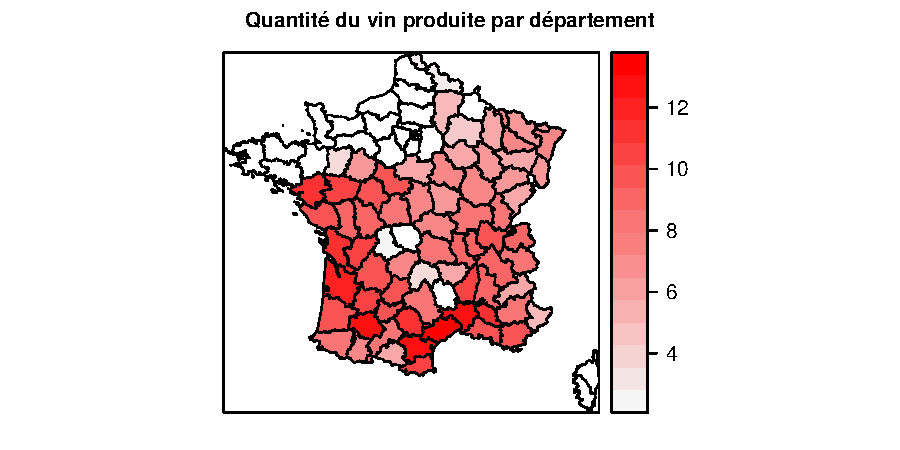
\includegraphics{note2pres_files/figure-latex/unnamed-chunk-18-1} 

}

\caption{Les quantité du vin non-IG moyennes par département}\label{fig:unnamed-chunk-18}
\end{figure}

\FloatBarrier

Puis, nous observons le comportement du reste des variables (les
representations graphiques sont grouppés dans l'annexe X). L'indice des
prix se comporte pratiquement comme quantité du vin produite, car cet
indice fut construit par biais de cette variable. Les autres moyennes ne
semblent pas avoir des structures corrélés dans l'espace au niveau de la
France. Dans notre analyse nous nous laissons liberté d'ignorer les
effets possibles d'autocorrelation spatiale dans nos données, parce que
au moment de constructions de notre base des données nous avons ignoré
les département ne produisant pas le vin simple, mais qui peuvent quand
même jouer son rôle si nous étions à prendre en compte la structure
spatiale des nos données.

\hypertarget{etude-de-la-variance}{%
\subsection{Etude de la variance}\label{etude-de-la-variance}}

Passons maintenant à l'étude de la variance. Nous allons décortiquer la
variance par type (between et within) afin d'obtenir une idée sur le
choix preferable de la dimention d'aggregation des nos données, car il
peut se reveler que la théorie ne corresponde pas à la réalitée (ex:
nous faisons face aux effets fixes par année et non par département).

Le tableau suivant regrouppe les statistiques déscriptives essentielles
:

\begin{itemize}
\tightlist
\item
  Moyennes
\item
  Variance sur l'échantillon complet
\item
  Variance \emph{between}
\item
  Variance \emph{within}
\end{itemize}

\FloatBarrier

\begin{table}[!htbp] \centering 
  \caption{Etude de la variance} 
  \label{} 
\begin{tabular}{@{\extracolsep{5pt}} ccccc} 
\\[-1.8ex]\hline 
\hline \\[-1.8ex] 
 & Mean & Overall & Between & Within \\ 
\hline \\[-1.8ex] 
Index prix & $1.431$ & $1.339$ & $1.012$ & $0.883$ \\ 
Index pesticides & $1.257$ & $0.483$ & $0.335$ & $0.350$ \\ 
Surface & $4.892$ & $1.986$ & $1.955$ & $0.410$ \\ 
Revenus & $9.891$ & $0.061$ & $0.061$ & $0.011$ \\ 
Temps & $3$ & $1.416$ & $0$ & $1.416$ \\ 
\hline \\[-1.8ex] 
\end{tabular} 
\end{table}

\FloatBarrier

Il est facile a rémarquer que la variance \emph{between} est plus
significative que la variance \emph{within}. Cela nous amêne à l'idée
qu'il faut utiliser un modèle qui permettra estimer et corriger ces
inégalités entre les individus, car nous sommes plus interessés par des
effets individuels moyens (les effets moyens pour tous les
départemetns). Ce qui est completement conforme à notre hypothèse qu'on
a exprimé lors de la formalisation du modèle économique théorique.

De plus, il est interessant d'observer les résultats obtenus pour le
test de Chow comparant le modèle complet (\emph{pooled model}) contre
les modèles au effet fixes et randomes. Le tableau suivant régrouppe les
p-valeurs de ce test pour les modèles univariées differents.

\FloatBarrier

\begin{table}[!htbp] \centering 
  \caption{Les p-valeurs de pooling-test de Chow} 
  \label{} 
\begin{tabular}{@{\extracolsep{5pt}} ccc} 
\\[-1.8ex]\hline 
\hline \\[-1.8ex] 
 & Random & Fixed \\ 
\hline \\[-1.8ex] 
Index prix & $0$ & $0$ \\ 
Index pesticides & $0.354$ & $0.294$ \\ 
Surface & $0$ & $0.0001$ \\ 
Revenus & $0.297$ & $0.247$ \\ 
\hline \\[-1.8ex] 
\end{tabular} 
\end{table}

\FloatBarrier

Sauf le cas de la surface nous ne pouvons pas rejeter l'hypothese nulle,
specifiant que les individus ont des effets identiques pour toute la
population.

\hypertarget{letude-des-types-deffets}{%
\subsection{L'étude des types d'effets}\label{letude-des-types-deffets}}

Nous avons déjà vu, qu'il est fortement probable que nous faisons face à
un modèle aux effets fixes individuelles. Il faut quand même le
justifier. Pour faire cela, nous allons effectuer le test de
multiplicateur de Lagrange sur la nature des effets (individuels,
temporels ou en double dimention). Selon les résultats des tests il est
difficile de choisir arbitrairement un type des effets. Il est évidente
que nous avons des effets fixes au niveau individuel ou des fixes en
double dimention pour toutes les variables.

\FloatBarrier

\begin{table}[!htbp] \centering 
  \caption{p-valeurs de Lagrange multiplier test} 
  \label{} 
\begin{tabular}{@{\extracolsep{5pt}} cccc} 
\\[-1.8ex]\hline 
\hline \\[-1.8ex] 
 & Individual & Time & Twoways \\ 
\hline \\[-1.8ex] 
Index prix & $0$ & $0.256$ & $0$ \\ 
Index pesticides & $0$ & $0.229$ & $0$ \\ 
Surface & $0$ & $0.030$ & $0$ \\ 
Revenus & $0$ & $0.248$ & $0$ \\ 
\hline \\[-1.8ex] 
\end{tabular} 
\end{table}

\FloatBarrier

Selon les résultats obtenus, ainsi que les evidences théoriques des
études anterieurs nous décidons de ne garder que les effets fixes au
niveau individuel afin de faciliter l'analyse.

\hypertarget{lanalyse-de-la-correlation}{%
\subsection{L'analyse de la
correlation}\label{lanalyse-de-la-correlation}}

Dans le tableau ci-dessous nous presentons les correlations des
variables après la correction pour les effets fixes individuels (nous
effectuons la transformation \emph{within} sur nos données en
substrayant les moyennes individuelles pour l'ensemble des variables).
Dans les annexes nous proposons egalement un tableau de correlation pour
les données non-transformées, ce qui permet d'observer les inégalités et
une pauvre répresentativitée des liens entres les variables pour les
données initiales.

Particulierement nous pouvons remarquer une forte correlation entre la
quantité offerte et le prix d'équilibre. Egalement \ldots{}

\hypertarget{modelisation}{%
\section{6. Modèlisation}\label{modelisation}}

\noindent

\rule[0.5ex]{\linewidth}{1pt}

\textcolor{red}{Séparer les modèles (OLS, 3SLS avec justification par 2SLS et la comparaison avec i3SLS, clusters en OLS et 3SLS).}

\textcolor{red}{Justifier le choix des modèles par 3 cas théoriques. Discuter les avantages et les inconveniences}

\textcolor{red}{Ajouter des liens avec des études méthodologiques precedents.}

\textcolor{red}{Pour le modèle 2SLS préciser la forme, tester les instruments}

\textcolor{red}{Arbitrage du choix de 2SLS vs 3SLS}

\noindent

\rule[0.5ex]{\linewidth}{1pt}

Cette partie du travail abordera la formulation économétrique du notre
problème. Nous allons débuter par la présentation des notions théoriques
implimentés dans ce travail, suivis par la formalisation économétrique
du modèle théorique que nous avons spécifié dans la séction 5. Après,
nous expliquerons la stratégie d'identification utilisée.

\hypertarget{presentation-de-la-methodologie}{%
\subsection{Presentation de la
méthodologie}\label{presentation-de-la-methodologie}}

L'AIDS (\emph{almost ideal demand system}) et les autres modèles de
demande cités dans la littérature ont de nombreuses lacunes qui les
rendent impropres pour l'estimation du marché du vin, selon Cembalo,
Caracciolo, and Pomarici (2014). Quand même, dans notre étude nous
allons utiliser un approche similaire à ce modèle là, sous des
suppositions restrictives.

Ce modèle nous permettra de simuler l'équilibre sur le marché du vin,
prenant ainsi en compte la pluspart des facteurs incitant les
producteurs du vin d'utiliser les pésticides.

\hypertarget{modele-econometrique}{%
\subsection{Modèle économétrique}\label{modele-econometrique}}

Dans cette séction nous allons presenter une par une nos modèles
économétriques correspondant chacune à un des trois cadres théoriques
possibles. Tous les modèles visent à estimer les effets moyenns pour
tous les départements sous des hypothèses differentes du fonctionnement
du marché. Dans tous les cas, l'aggregation des effets au niveau
national (ou au niveau des grouppes) nous permet de mitiger les biais
eventuels, liés à la misspecification du modèle.

Pour le cadre où nous n'observons pas des interactions entre la demande
et l'offre sur le marché (M1), nous ésimons un modèle simple. Nous
écrivons notre modèle sous la forme suivante :

\begin{equation*}
  qo_{i,t} = a_1 + b Po_{i,t} + c X_{i,t} + u_{i,t}
\end{equation*}

A ce point nous avons un choix : soit nous supposons que les
agriculteurs sont des preneurs des prix, ce qui nous permet de traiter
le prix comme une variable exogène; soit nous dévrions construire un
estimateur IV afin de traiter l'endogénéité eventuelle de l'index des
prix. Evidement le premier cas est le plus simple, mais pour justifier
l'implementation de cette méthode nous dévrions effectuer des tests
d'énogénéité des prix. Le deuxième cas est beaucoup plus réaliste,
puisque les viticulteurs sont rarement preneurs des prix et l'offre
aussi joue son rôle sur l'équilibre du marché.

Dans la dérnier situation nous utilisons les idées de MacKay and Miller
(2018), supposant que les variables détérminant la demande sont des
instruments fiables pour la prédiction des variables endogènes dans
l'équation d'offre (bien que dans notre cas nous ignorons les effets des
intéractions entre l'offre et la demande). Particulieremnt ici nous
pourrions utiliser les données sur les revenus afin d'instrumenter le
niveau des prix (l'indice des prix du vin).

Passons maintenant au modèle plus complexe (M2), basé sur l'hypothèse
que la demande influence l'offre, affectant également le mode
d'utilisation des pésticides par les agriculteurs. Nous pouvons réécrire
notre système d'equations dans ce cas sous la forme suivante :

\begin{align*}
  qo_{i,t} & = a_1 + b Po_{i,t} + c X_{i,t} + u_{i,t} \\ 
  qd_{i,t} & = \alpha_{i} + \beta Pd_{i,t} + \gamma Z_{i,t} + \epsilon_{i,t}  \\
\end{align*}

Nous posons que l'offre et la demande sont egaux au niveau de
département : \(qd_{i,t} = qo_{i,t}\). C'est à dire l'offre interne du
département vise à satisfaire la demande interne du même département.

En termes d'aggregation ex-post des effets estimés, nous sommes sensé de
tomber sur l'équilibre au niveau du marché national. En d'autre mots, le
système (qui implique : \(Qd = Qo\)) :

\begin{equation*}
  qd_{i,t} = qo_{i,t}
\end{equation*}

Au point d'équilibre nous rencontrons également l'égalité des prix :

\begin{equation*}
  Po_{1,t} = Pd_{1,t}
\end{equation*}

De cette façon nous obtenons un système des systèmes des équations. En
simplifiant l'écriture nous pouvons la representer sous la forme
suivante :

\begin{align*}
  q_{i,t} & = \alpha_{i} + \beta P_{i,t} + \gamma Z_{i,t} + \epsilon_{i,t} \\
  q_{i,t} & = a_i + b P_{i,t} + c X_{i,t} + u_{i,t}
\end{align*}

Et finalement, nous pouvons estimer les deux modèles (M1 et M2) en
regrouppant les département par leurs caractéristiques. Appelons ces
modèles M3.1 et M3.2 réspectivement.

Le prémiér prénant la forme :

\begin{align*}
  qo_{i,t} & = a_1 + b Po_{i,t} + c X_{i,t} + u_{i,t} \\ 
\end{align*}

Tandis que le dérnier :

\begin{align*}
  q_{i_{c},t} & = \alpha_{i_{c}} + \beta P_{i_{c},t} + \gamma Z_{i_{c},t} + \epsilon_{i_{c},t} \\
  q_{i_{c},t} & = a_i + b P_{i_{c},t} + c X_{i_{c},t} + u_{i_{c},t}
\end{align*}

Avec \(c\) décrivant l'appartenance de département à un des clusters.

Pour finir cette partie, resumons que nous avons à notre disposition
plusieurs chemins differents à traiter ce modèle du point de vue
économétrique. Le plus simple est d'estimer les effets des pésticides
sur l'offre du vin en ignorant les impacts du comportement des
consommaterus sur les producteurs. Cette méthode implique une éstimation
par OLS simples (ou IV-OLS, lesquels introduisent la notion
d'éndogénéité des prix). D'autre coté, nous pouvons implementer les
tripples moindre carrés (nous dévrions comparer les résultats obtenus
avec un système des équations non-réliées, éstimé par 2SLS afin de
traiter l'éndogenèité), qui nous permettrons d'obtenir des résultats
identiques aux résultats d'estimations des équation structurelles sous
l'hypothèse des intéractions entre l'offre et la demande. Cette méthode
offre la possibilité d'estimer le système d'équations avec plusieurs
variables endogèenes en prenant en compte les deux coté du marché à la
fois. Finalement, si on trouve qu'il y existe une heterogeneité entre
les départements en termes d'équilibre interne, nous pourrions réestimer
les modèles en clusterisant nos \emph{individus} (départements) par des
differents classes selon leurs attributs, pour après estimer les
equations par cluster.

\hypertarget{hypotheses-sur-le-comportement-des-estimateurs}{%
\subsection{Hypothèses sur le comportement des
estimateurs}\label{hypotheses-sur-le-comportement-des-estimateurs}}

Nous attendons à ce que l'éstimateur de 3SLS, qui permet de capter les
effets de correlations entre les équation en presence de plusieures
variables exogènes nous permettra d'obtenir des estimations les plus
fiables. Cette méthode nous permet à depasser le biais de simultanéité
qui apparaisse dans le cas d'estimation des systèmes d'équations liées
(dans notre cas nous étudions les effets des pésticides sur l'offre et
production du vin simple sous hypothèse de présence des effets du
marché). L'estimateur pareil donne des résultats similaires à
l'éstimateur de ILS (\emph{indirect least squares}). De plus, sa version
iterée (qui converge à des résultats similaires à ceux obtenus par
l'éstimation avec maximum de vraisamblance) donne des résultats avec la
moindre variance.

Les propriétés de cet éstimateurs sont :

\begin{itemize}
\tightlist
\item
  Consistence ;
\item
  Efficience (asymptotique) ;
\item
  La distribuitions pour les estimateurs suit une loi normale suelement
  dans des grands échantillons.
\end{itemize}

Quand même dès le debut nous envisageons que cet éstimateur ne refletera
pas la nature du marché. C'est pourquoi nous, dans ce travail, testons
plusieurs modèles.

Parmis les inconveniences eventuelles on a également la faible
representation des effets hetérogenes entre les départements par le
modèle. Nous estimons seulemnt les effets moyens et ainsi ignorons les
differences des élasticités pour des départements differents.
Hereusement ce problème peut être rémédiée par l'introduction des
clusters, regrouppant des département ayant le comportement similaire.

Finalement, il existe des effets qu'on ignore completement, mais qui
risquent d'intervenir. Par example, nous ignorons la présence
d'autocorrelation spatiale et/ou temporelle dans notre modèle.
Egalement, un nombre probablement insuffisant des facteurs est utilisé
dans ce modèle, ce qui risaue d'apporter le biais des variables omises
dans nos estimations.

\hypertarget{resultats-des-estimations}{%
\section{7. Résultats des estimations}\label{resultats-des-estimations}}

Dans cette séction nous allons presenter les résultats économétriques
pour des differents modèles ainsi que les comparer.

Nous estimons l'enseble des differents modèles possibles afin de pouvoir
choisir la méthode la plus raisonnable. Les modèles suivantes sont
traitées séparement :

\begin{itemize}
\tightlist
\item
  M1 : modèle simple sans intéractions entre l'offre et la demande ;
\item
  M2 : modèle complexe visant à integrer les intéractions entre l'offre
  et la demande en presence des variables éndogènes ;
\item
  M3 : les modèles sur les données clustérisés (M3.1 et M3.2
  réspectivement pour les deux cas précedents).
\end{itemize}

\hypertarget{m1-les-resultats-en-absence-des-interactions}{%
\subsection{M1 : Les résultats en absence des
intéractions}\label{m1-les-resultats-en-absence-des-interactions}}

\FloatBarrier

\begin{table}[!htbp]
\begin{center}
\begin{tabular}{l c c }
\hline
 & OLS & IV-OLS \\
\hline
ipi        & $0.30^{***}$  & $-0.28$      \\
           & $(0.02)$      & $(0.25)$     \\
si         & $0.23^{***}$  & $0.47^{***}$ \\
           & $(0.04)$      & $(0.13)$     \\
iki        & $-0.16^{***}$ & $-0.11$      \\
           & $(0.05)$      & $(0.09)$     \\
\hline
R$^2$      & 0.52          & -0.87        \\
Adj. R$^2$ & 0.52          & -0.89        \\
Num. obs.  & 345           & 345          \\
RMSE       & 0.29          & 0.58         \\
\hline
\multicolumn{3}{l}{\scriptsize{$^{***}p<0.001$, $^{**}p<0.01$, $^*p<0.05$}}
\end{tabular}
\caption{Statistical models}
\label{table : ols et ivols}
\end{center}
\end{table}

\FloatBarrier

\hypertarget{m2-les-resultats-dans-le-cas-des-effets-du-marche-presents}{%
\subsection{M2 : Les résultats dans le cas des effets du marché
presents}\label{m2-les-resultats-dans-le-cas-des-effets-du-marche-presents}}

Dans cette séction nous allons étudier le modèle sous l'hypothèse de
présence des effets de la conjoncture sur les décisions des
agriculteurs. Nous allons comparér des résultats des plusieurs modèles
afin de verifier sa validité.

Le modèle \ldots{} 3SLS \ldots{}

Afin de contracter la variance des estimateurs \ldots{} i3SLS \ldots{}
Cette méthode nous donne des résultats similaire à ceux obtenus par FIML
\ldots{}

Nous comparons les résultats obtenus avec le modèle en absence des
intéractions (sous l'hypothèse que les résidus des deux équations ont
une correlation nulle) \ldots{} 2SLS \ldots{} . Ce méthode donne des
résultats équivalents à ILS \ldots{}

Les résultats sont régrouppé sous format d'un tableau \ldots{}

\FloatBarrier

\begin{table}[!htbp]
\begin{center}
\begin{tabular}{l c c c }
\hline
 & 2SLS & 3SLS & i3SLS \\
\hline
Demande: ipi        & $0.79^{***}$   & $0.79^{***}$   & $0.79^{***}$   \\
                    & $(0.15)$       & $(0.15)$       & $(0.15)$       \\
Demande: ri         & $-13.07^{***}$ & $-13.07^{***}$ & $-13.07^{***}$ \\
                    & $(2.76)$       & $(2.76)$       & $(2.76)$       \\
Offre: ipi          & $-0.28$        & $-0.25$        & $-0.25$        \\
                    & $(0.25)$       & $(0.25)$       & $(0.24)$       \\
Offre: si           & $0.47^{***}$   & $0.45^{***}$   & $0.45^{***}$   \\
                    & $(0.13)$       & $(0.13)$       & $(0.12)$       \\
Offre: iki          & $-0.11$        & $-0.17^{*}$    & $-0.17^{*}$    \\
                    & $(0.09)$       & $(0.08)$       & $(0.08)$       \\
\hline
Demande: R$^2$      & -0.41          & -0.41          & -0.41          \\
Offre: R$^2$        & -0.87          & -0.74          & -0.75          \\
Demande: Adj. R$^2$ & -0.42          & -0.42          & -0.42          \\
Offre: Adj. R$^2$   & -0.89          & -0.75          & -0.76          \\
Num. obs. (total)   & 690            & 690            & 690            \\
\hline
\multicolumn{4}{l}{\scriptsize{$^{***}p<0.001$, $^{**}p<0.01$, $^*p<0.05$}}
\end{tabular}
\caption{Statistical models}
\label{table : 2sls, 3sls and fiml}
\end{center}
\end{table}

\FloatBarrier

\hypertarget{m3-les-resultats-pour-des-departements-grouppes}{%
\subsection{M3 : Les résultats pour des départements
grouppés}\label{m3-les-resultats-pour-des-departements-grouppes}}

\hypertarget{clusterisation}{%
\subsubsection{Clusterisation}\label{clusterisation}}

\hypertarget{between}{%
\paragraph{\texorpdfstring{\emph{Between}}{Between}}\label{between}}

Nous avons vus dans le comportement des résidus une nature non-aléatoire
grouppé. Cela nous amène à l'idée de construire k-clusters pour
modèliser les rélations par grouppe.

Nous supposons que les départements ayant des valeurs moyennes
interannuelles proches (transformation Between) ont le comportement
identique. La clusterisation est effectué sur les données Between pour
les départements.

Nous povons supposer que le nombre des clusters optimal est entre 3 et
5. Prenant en compte les graphiques des résidus vus lros d'analse des
modèles nous allons supposer qu'il n'y a que 3 clusters principaux.

\hypertarget{within}{%
\paragraph{\texorpdfstring{\emph{Within}}{Within}}\label{within}}

Nous avons vus dans le comportement des résidus une nature non-aléatoire
grouppé. Cela nous amène à l'idée de construire k-clusters pour
modèliser les rélations par grouppe.

D'abord on compare le comportement des cluster pour les données à
l'information complete et les données Within.

Comme nous pouvons voir dans les résultats le nombre des cluster
optimaux est trop large pour les séparer dans l'analyse.

\hypertarget{between-et-within}{%
\paragraph{\texorpdfstring{\emph{Between} et
\emph{Within}}{Between et Within}}\label{between-et-within}}

Dans le cas d'information complete on a :

Nous povons supposer que le nombre des clusters optimal est entre 3 et
5. Prenant en compte les graphiques des résidus vus lros d'analse des
modèles nous allons supposer qu'il n'y a que 3 clusters principaux.

\hypertarget{comparaison-des-differentes-methodes}{%
\paragraph{Comparaison des differentes
méthodes}\label{comparaison-des-differentes-methodes}}

Afin de pouvoir comparer des valeurs differents de WSS (\emph{within
summ of squares}) nous allons visualiser la valeur dun indice :

\begin{equation*}
    WSS^{'} = \frac{SS}{min(WSS)}
\end{equation*}

Ce qui nous permettra d'évaluer les écarts rélatives du WSS de sa valeur
minimale (pour nombre des clusters égal à 15).

\FloatBarrier

\begin{center}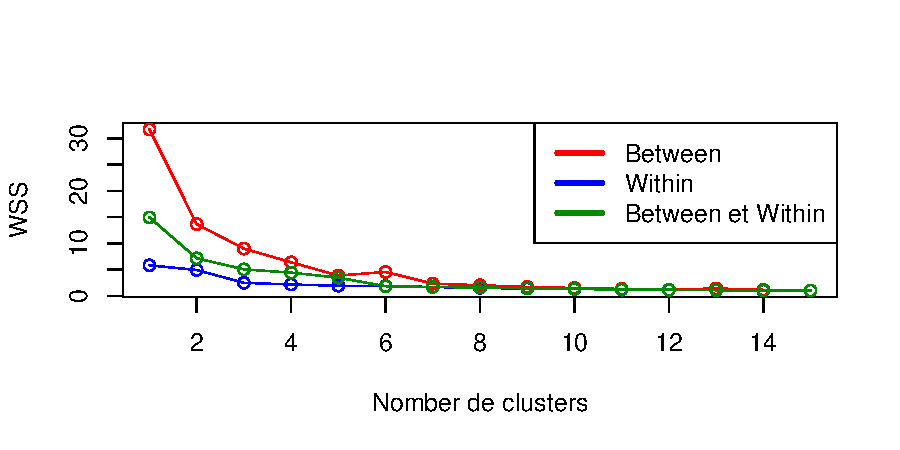
\includegraphics{note2pres_files/figure-latex/unnamed-chunk-41-1} \end{center}

\FloatBarrier

Pour la transformation \emph{within} nous observons la convergence la
plus vite vers la valeure minimale de WSS.

\hypertarget{m3.1-le-cadre-en-absence-des-interaction-avec-la-demande}{%
\subsubsection{M3.1 : Le cadre en absence des intéraction avec la
demande}\label{m3.1-le-cadre-en-absence-des-interaction-avec-la-demande}}

\FloatBarrier

\begin{table}[!htbp]
\begin{center}
\begin{tabular}{l c c c c c c }
\hline
 & Model 1 & Model 2 & Model 3 & Model 4 & Model 5 & Model 6 \\
\hline
ipi        & $0.15$   & $0.15$   & $0.51^{***}$ & $0.22^{*}$  & $0.69^{***}$  & $4.36$   \\
           & $(0.04)$ & $(0.04)$ & $(0.02)$     & $(0.10)$    & $(0.03)$      & $(4.60)$ \\
si         & $-0.54$  & $-0.59$  & $0.09^{*}$   & $0.19^{**}$ & $0.19^{***}$  & $-0.69$  \\
           & $(0.58)$ & $(0.58)$ & $(0.04)$     & $(0.07)$    & $(0.04)$      & $(1.14)$ \\
iki        & $7.58$   & $7.73$   & $-0.11^{*}$  & $-0.01$     & $-0.16^{***}$ & $0.14$   \\
           & $(4.62)$ & $(4.65)$ & $(0.04)$     & $(0.07)$    & $(0.04)$      & $(0.52)$ \\
\hline
R$^2$      & 0.92     & 0.92     & 0.79         & 0.55        & 0.76          & -15.69   \\
Adj. R$^2$ & 0.80     & 0.80     & 0.78         & 0.54        & 0.76          & -15.95   \\
Num. obs.  & 5        & 5        & 145          & 145         & 195           & 195      \\
RMSE       & 0.39     & 0.39     & 0.14         & 0.21        & 0.23          & 1.96     \\
\hline
\multicolumn{7}{l}{\scriptsize{$^{***}p<0.001$, $^{**}p<0.01$, $^*p<0.05$}}
\end{tabular}
\caption{Statistical models}
\label{table : ols et ivols clusters}
\end{center}
\end{table}

\FloatBarrier

\hypertarget{m3.2-le-cadre-dinterference-avec-la-demande}{%
\subsubsection{M3.2 : Le cadre d'interference avec la
demande}\label{m3.2-le-cadre-dinterference-avec-la-demande}}

Nous evaluons le système en introduisant les variables de grouppe (dummy
variables) sous l'hypothèse des résidus joints.

Cluster 1

\FloatBarrier

\begin{table}[!htbp]
\begin{center}
\begin{tabular}{l c c c }
\hline
 & 2SLS & 3SLS & i3SLS \\
\hline
Demande: ipi        & $0.12^{*}$ & $0.12^{*}$ & $0.12^{*}$ \\
                    & $(0.03)$   & $(0.03)$   & $(0.03)$   \\
Demande: ri         & $18.43$    & $18.43$    & $18.43$    \\
                    & $(14.62)$  & $(14.62)$  & $(14.62)$  \\
Offre: ipi          & $0.15$     & $0.16^{*}$ & $0.17$     \\
                    & $(0.04)$   & $(0.04)$   & $(0.06)$   \\
Offre: si           & $-0.59$    & $-0.69$    & $-0.79$    \\
                    & $(0.58)$   & $(0.58)$   & $(0.92)$   \\
Offre: iki          & $7.73$     & $4.99$     & $2.08$     \\
                    & $(4.65)$   & $(3.93)$   & $(5.48)$   \\
\hline
Demande: R$^2$      & 0.88       & 0.88       & 0.88       \\
Offre: R$^2$        & 0.92       & 0.89       & 0.79       \\
Demande: Adj. R$^2$ & 0.84       & 0.84       & 0.84       \\
Offre: Adj. R$^2$   & 0.84       & 0.78       & 0.59       \\
Num. obs. (total)   & 10         & 10         & 10         \\
\hline
\multicolumn{4}{l}{\scriptsize{$^{***}p<0.001$, $^{**}p<0.01$, $^*p<0.05$}}
\end{tabular}
\caption{Statistical models}
\label{table : 2sls, 3sls and fiml cluster 1}
\end{center}
\end{table}

\FloatBarrier

Cluster 2

\FloatBarrier

\begin{table}[!htbp]
\begin{center}
\begin{tabular}{l c c c }
\hline
 & 2SLS & 3SLS & i3SLS \\
\hline
Demande: ipi        & $0.66^{***}$  & $0.66^{***}$  & $0.66^{***}$  \\
                    & $(0.11)$      & $(0.11)$      & $(0.11)$      \\
Demande: ri         & $-6.68^{***}$ & $-6.68^{***}$ & $-6.68^{***}$ \\
                    & $(1.95)$      & $(1.95)$      & $(1.95)$      \\
Offre: ipi          & $0.22^{*}$    & $0.20^{*}$    & $0.20$        \\
                    & $(0.10)$      & $(0.10)$      & $(0.10)$      \\
Offre: si           & $0.19^{**}$   & $0.18^{*}$    & $0.18^{*}$    \\
                    & $(0.07)$      & $(0.07)$      & $(0.07)$      \\
Offre: iki          & $-0.01$       & $0.03$        & $0.03$        \\
                    & $(0.07)$      & $(0.07)$      & $(0.07)$      \\
\hline
Demande: R$^2$      & 0.77          & 0.77          & 0.77          \\
Offre: R$^2$        & 0.55          & 0.52          & 0.52          \\
Demande: Adj. R$^2$ & 0.77          & 0.77          & 0.77          \\
Offre: Adj. R$^2$   & 0.54          & 0.52          & 0.52          \\
Num. obs. (total)   & 290           & 290           & 290           \\
\hline
\multicolumn{4}{l}{\scriptsize{$^{***}p<0.001$, $^{**}p<0.01$, $^*p<0.05$}}
\end{tabular}
\caption{Statistical models}
\label{table : 2sls, 3sls and fiml cluster 2}
\end{center}
\end{table}

\FloatBarrier

Cluster 3

\FloatBarrier

\begin{table}[!htbp]
\begin{center}
\begin{tabular}{l c c c }
\hline
 & 2SLS & 3SLS & i3SLS \\
\hline
Demande: ipi        & $1.35^{***}$  & $1.35^{***}$  & $1.35^{***}$  \\
                    & $(0.27)$      & $(0.27)$      & $(0.27)$      \\
Demande: ri         & $-10.08^{**}$ & $-10.08^{**}$ & $-10.08^{**}$ \\
                    & $(3.51)$      & $(3.51)$      & $(3.51)$      \\
Offre: ipi          & $4.36$        & $4.71$        & $4.75$        \\
                    & $(4.60)$      & $(4.58)$      & $(5.06)$      \\
Offre: si           & $-0.69$       & $-0.68$       & $-0.68$       \\
                    & $(1.14)$      & $(1.14)$      & $(1.26)$      \\
Offre: iki          & $0.14$        & $0.43$        & $0.46$        \\
                    & $(0.52)$      & $(0.38)$      & $(0.42)$      \\
\hline
Demande: R$^2$      & 0.26          & 0.26          & 0.26          \\
Offre: R$^2$        & -15.69        & -19.07        & -19.44        \\
Demande: Adj. R$^2$ & 0.25          & 0.25          & 0.25          \\
Offre: Adj. R$^2$   & -15.87        & -19.27        & -19.65        \\
Num. obs. (total)   & 390           & 390           & 390           \\
\hline
\multicolumn{4}{l}{\scriptsize{$^{***}p<0.001$, $^{**}p<0.01$, $^*p<0.05$}}
\end{tabular}
\caption{Statistical models}
\label{table : 2sls, 3sls and fiml cluster 3}
\end{center}
\end{table}

\FloatBarrier

\hypertarget{conclusions}{%
\section{9. Conclusions}\label{conclusions}}

\begin{itemize}
\tightlist
\item
  Le marché du vin
\item
  Le rôle des pésticides\\
\item
  Validité
\end{itemize}

\FloatBarrier

\hypertarget{le-marche-du-vin}{%
\subsection{Le marché du vin}\label{le-marche-du-vin}}

\begin{itemize}
\tightlist
\item
  Un comportement inattendus

  \begin{itemize}
  \item
    Les effets de substitution contre les produits de la haute gamme
  \item
    Les effets négatives du revenu
  \item
  \end{itemize}
\end{itemize}

\FloatBarrier

\hypertarget{le-role-des-pesticides}{%
\subsection{Le rôle des pésticides}\label{le-role-des-pesticides}}

\begin{itemize}
\tightlist
\item
  Confirmation des résultats des études précedentes

  \begin{itemize}
  \tightlist
  \item
    Utilisés pour réduire les pertes
  \end{itemize}
\end{itemize}

\FloatBarrier

\hypertarget{validite}{%
\subsection{Validité}\label{validite}}

\begin{itemize}
\tightlist
\item
  Faible validité du modèle économétrique

  \begin{itemize}
  \tightlist
  \item
    Variables ommises
  \end{itemize}
\end{itemize}

\FloatBarrier

\newpage

\hypertarget{annexes}{%
\section{Annexes}\label{annexes}}

\hypertarget{a-les-statistiques-descriptives}{%
\subsection{A Les statistiques
déscriptives}\label{a-les-statistiques-descriptives}}

\hypertarget{a1-les-moyennes-par-departement}{%
\subsubsection{A1 Les moyennes par
département}\label{a1-les-moyennes-par-departement}}

\FloatBarrier

\begin{figure}[!htbp]

{\centering 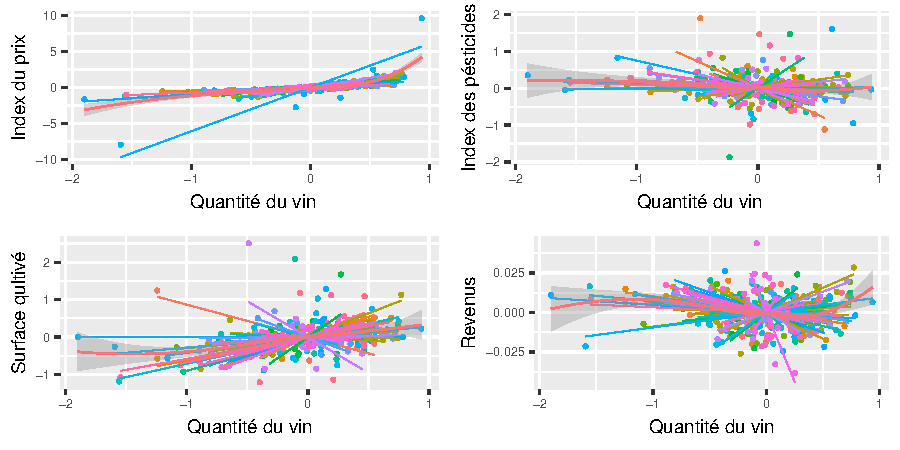
\includegraphics{note2pres_files/figure-latex/unnamed-chunk-53-1} 

}

\caption{Les valeurs moyennes par département}\label{fig:unnamed-chunk-53}
\end{figure}

\FloatBarrier

\newpage

\hypertarget{a2-les-graphiques-bivaries}{%
\subsubsection{A2 Les graphiques
bivariés}\label{a2-les-graphiques-bivaries}}

\hypertarget{cas-general}{%
\paragraph{Cas général}\label{cas-general}}

\FloatBarrier

\begin{figure}[!htbp]

{\centering \includegraphics{note2pres_files/figure-latex/unnamed-chunk-54-1} 

}

\caption{L'étude bivarié}\label{fig:unnamed-chunk-54}
\end{figure}

\FloatBarrier

\hypertarget{transformation-within}{%
\paragraph{\texorpdfstring{Transformation
\emph{Within}}{Transformation Within}}\label{transformation-within}}

\FloatBarrier

\begin{figure}[!htbp]

{\centering 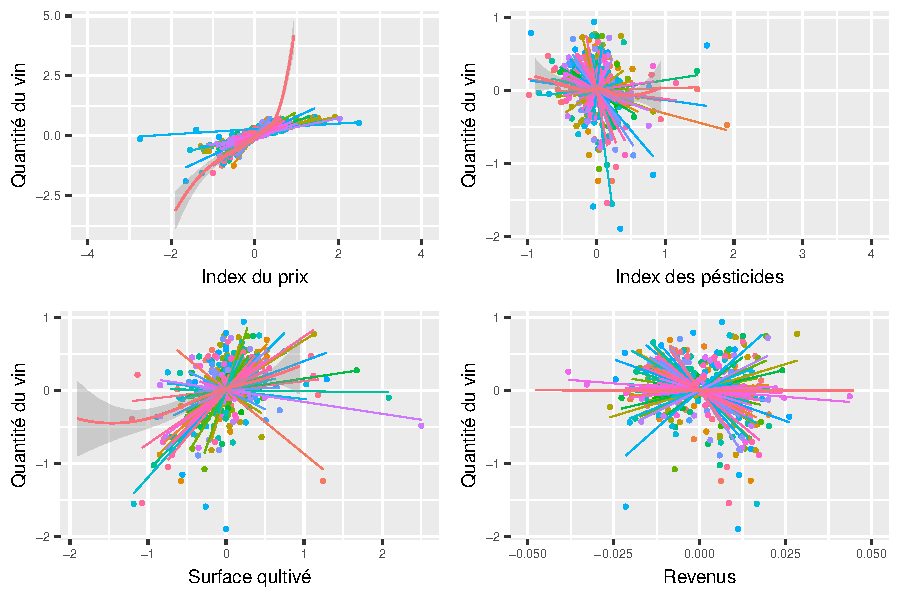
\includegraphics{note2pres_files/figure-latex/unnamed-chunk-55-1} 

}

\caption{Rélations bivariés dans le cas de transformation within}\label{fig:unnamed-chunk-55}
\end{figure}

\FloatBarrier

\newpage

\hypertarget{a3-la-correlation}{%
\subsubsection{A3 La correlation}\label{a3-la-correlation}}

\hypertarget{cas-general-1}{%
\paragraph{Cas général}\label{cas-general-1}}

Le premier tableau combrend les résultats pour les données
telles-quelles, le deuxieme par contre integre les résultats pour les
données sous la trasformation \emph{within}.

\FloatBarrier

\begin{longtable}[]{@{}lrrrrrr@{}}
\toprule
& Quantité du vin & IP & Surface & Revenus & Index pésticides &
Temps\tabularnewline
\midrule
\endhead
Quantité du vin & 1.0000 & 0.0177 & 0.9559 & -0.0266 & -0.0667 &
-0.0360\tabularnewline
IP & 0.0177 & 1.0000 & -0.0513 & 0.0065 & -0.0590 &
0.1082\tabularnewline
Surface & 0.9559 & -0.0513 & 1.0000 & -0.0567 & -0.0486 &
-0.0640\tabularnewline
Revenus & -0.0266 & 0.0065 & -0.0567 & 1.0000 & -0.0433 &
0.1188\tabularnewline
Index pésticides & -0.0667 & -0.0590 & -0.0486 & -0.0433 & 1.0000 &
0.2971\tabularnewline
Temps & -0.0360 & 0.1082 & -0.0640 & 0.1188 & 0.2971 &
1.0000\tabularnewline
\bottomrule
\end{longtable}

\FloatBarrier

\hypertarget{transformation-within-1}{%
\paragraph{\texorpdfstring{Transformation
\emph{Within}}{Transformation Within}}\label{transformation-within-1}}

Les rélations entre les variables mieux ressortent pour les données
transformées.

\FloatBarrier

\begin{longtable}[]{@{}lrrrrrr@{}}
\toprule
& Quantité du vin & IP & Surface & Revenus & Index pésticides &
Temps\tabularnewline
\midrule
\endhead
Quantité du vin & 1.0000 & 0.6656 & 0.3655 & -0.1601 & -0.1813 &
-0.1994\tabularnewline
IP & 0.6656 & 1.0000 & 0.1862 & 0.1119 & -0.0108 & 0.1640\tabularnewline
Surface & 0.3655 & 0.1862 & 1.0000 & -0.1657 & -0.2035 &
-0.3103\tabularnewline
Revenus & -0.1601 & 0.1119 & -0.1657 & 1.0000 & 0.2103 &
0.6522\tabularnewline
Index pésticides & -0.1813 & -0.0108 & -0.2035 & 0.2103 & 1.0000 &
0.4100\tabularnewline
Temps & -0.1994 & 0.1640 & -0.3103 & 0.6522 & 0.4100 &
1.0000\tabularnewline
\bottomrule
\end{longtable}

\FloatBarrier

\newpage

\hypertarget{b-analyse-des-resultats-m1}{%
\subsection{B Analyse des résultats
M1}\label{b-analyse-des-resultats-m1}}

\hypertarget{b1-le-compoertement-des-residus}{%
\subsubsection{B1 Le compoertement des
résidus}\label{b1-le-compoertement-des-residus}}

\FloatBarrier

\begin{longtable}[]{@{}lrr@{}}
\toprule
& OLS & IV-OLS\tabularnewline
\midrule
\endhead
Vin & 0.6932 & 0.8783\tabularnewline
IP & 0.0000 & 0.8470\tabularnewline
Surface & 0.0000 & 0.0000\tabularnewline
Revenus & -0.2389 & 0.0000\tabularnewline
Pesticides & 0.0000 & 0.0000\tabularnewline
\bottomrule
\end{longtable}

\FloatBarrier

\FloatBarrier

\begin{figure}[!htbp]

{\centering 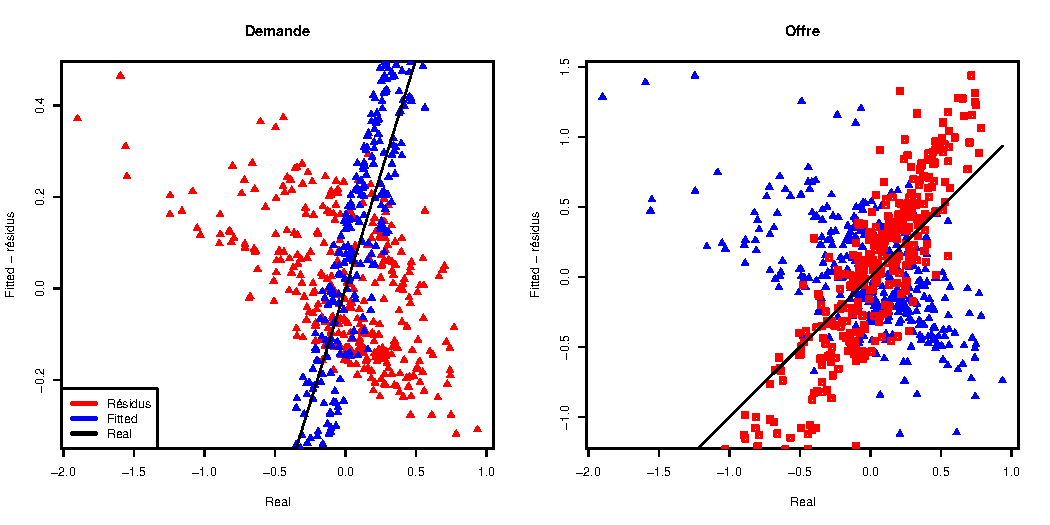
\includegraphics{note2pres_files/figure-latex/unnamed-chunk-62-1} 

}

\caption{Les résidus contre la variable prédite}\label{fig:unnamed-chunk-62}
\end{figure}

\FloatBarrier

\hypertarget{b2-lautocorrelation}{%
\subsubsection{B2 L'autocorrelation}\label{b2-lautocorrelation}}

\FloatBarrier

\begin{table}[!htbp] \centering 
  \caption{Les statistiques test de Durbin-Watson} 
  \label{} 
\begin{tabular}{@{\extracolsep{5pt}} ccc} 
\\[-1.8ex]\hline 
\hline \\[-1.8ex] 
 & OLS & IV-OLS \\ 
\hline \\[-1.8ex] 
Equation d'offre & $0.627$ & $0.637$ \\ 
\hline \\[-1.8ex] 
\end{tabular} 
\end{table}

\FloatBarrier

\hypertarget{b3-test-de-lheteroskedacite}{%
\subsubsection{B3 Test de
l'hétéroskedacité}\label{b3-test-de-lheteroskedacite}}

\FloatBarrier

\begin{table}[!htbp] \centering 
  \caption{Les résultat du test de Bartlett sur l'heteroscedacité} 
  \label{} 
\begin{tabular}{@{\extracolsep{5pt}} ccc} 
\\[-1.8ex]\hline 
\hline \\[-1.8ex] 
 & OLS & IV-OLS \\ 
\hline \\[-1.8ex] 
Equation d'offre & $0$ & $0$ \\ 
\hline \\[-1.8ex] 
\end{tabular} 
\end{table}

\FloatBarrier

\newpage

\hypertarget{b4-la-normalite-des-residus}{%
\subsubsection{B4 La normalité des
résidus}\label{b4-la-normalite-des-residus}}

\FloatBarrier

\FloatBarrier

\begin{table}[!htbp] \centering 
  \caption{Shapiro-Wilk test de normalité des résidus} 
  \label{} 
\begin{tabular}{@{\extracolsep{5pt}} ccc} 
\\[-1.8ex]\hline 
\hline \\[-1.8ex] 
 & OLS & IV-OLS \\ 
\hline \\[-1.8ex] 
Equation d'offre & $0$ & $0$ \\ 
\hline \\[-1.8ex] 
\end{tabular} 
\end{table}

\FloatBarrier

\FloatBarrier

\begin{figure}[!htbp]

{\centering 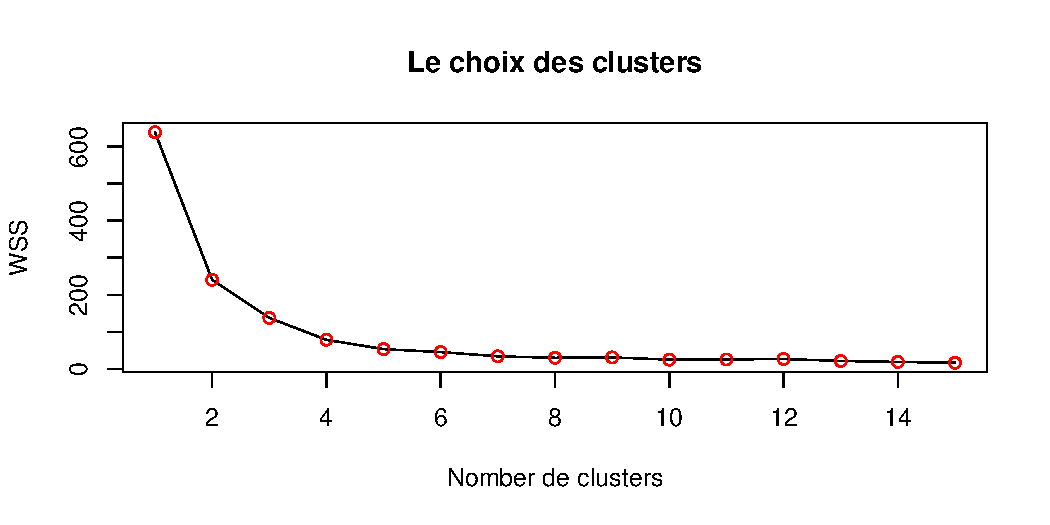
\includegraphics{note2pres_files/figure-latex/unnamed-chunk-69-1} 

}

\caption{Les PDF des résidus}\label{fig:unnamed-chunk-69}
\end{figure}

\FloatBarrier

\newpage

\hypertarget{b5-comparaisons-des-modeles}{%
\subsubsection{B5 Comparaisons des
modèles}\label{b5-comparaisons-des-modeles}}

\FloatBarrier

\begin{table}[!htbp] \centering 
  \caption{Diagnostiques d'estimateur IV} 
  \label{} 
\begin{tabular}{@{\extracolsep{5pt}} ccccc} 
\\[-1.8ex]\hline 
\hline \\[-1.8ex] 
 & df1 & df2 & statistic & p-value \\ 
\hline \\[-1.8ex] 
Weak instruments & 2 & 341 & 3.64540654308872 & 0.0271335957622741 \\ 
Wu-Hausman & 1 & 341 & 22.5532474455387 & 3.0150818630523e-06 \\ 
Sargan & 1 & - & 0 & 1 \\ 
\hline \\[-1.8ex] 
\end{tabular} 
\end{table}

\FloatBarrier

\newpage

\hypertarget{c-analyse-des-resultats-m2}{%
\subsection{C Analyse des résultats
M2}\label{c-analyse-des-resultats-m2}}

\hypertarget{c1-independance-des-residus}{%
\subsubsection{C1 Independance des
résidus}\label{c1-independance-des-residus}}

\FloatBarrier

\FloatBarrier

\FloatBarrier

\begin{figure}[!htbp]

{\centering \includegraphics{note2pres_files/figure-latex/unnamed-chunk-75-1} 

}

\caption{Les résidus contre la variable prédite}\label{fig:unnamed-chunk-75}
\end{figure}

\FloatBarrier

\FloatBarrier

\begin{figure}[!htbp]

{\centering \includegraphics{note2pres_files/figure-latex/unnamed-chunk-76-1} 

}

\caption{Les résidus et les prédictions, le cas de i3SLS}\label{fig:unnamed-chunk-76}
\end{figure}

\FloatBarrier

\newpage

\hypertarget{c2-lautocorrelation}{%
\subsubsection{C2 L'autocorrelation}\label{c2-lautocorrelation}}

\FloatBarrier

\begin{table}[!htbp] \centering 
  \caption{Les resultats du test de Durbin-Watson} 
  \label{} 
\begin{tabular}{@{\extracolsep{5pt}} cccc} 
\\[-1.8ex]\hline 
\hline \\[-1.8ex] 
 & 2SLS & 3SLS & i3SLS \\ 
\hline \\[-1.8ex] 
Equation de demande & $0.618$ & $0.618$ & $0.618$ \\ 
Equation d'offre & $0.637$ & $0.638$ & $0.638$ \\ 
\hline \\[-1.8ex] 
\end{tabular} 
\end{table}

\FloatBarrier

\hypertarget{c3-test-de-lheteroskedacite}{%
\subsubsection{C3 Test de
l'hétéroskedacité}\label{c3-test-de-lheteroskedacite}}

\FloatBarrier

\% Table created by stargazer v.5.2.2 by Marek Hlavac, Harvard
University. E-mail: hlavac at fas.harvard.edu \% Date and time: mar.,
déc. 24, 2019 - 20:06:34

\begin{table}[!htbp] \centering 
  \caption{Test de Bartlett sur l'heterockedacité} 
  \label{} 
\begin{tabular}{@{\extracolsep{5pt}} cccc} 
\\[-1.8ex]\hline 
\hline \\[-1.8ex] 
 & 2SLS & 3SLS & i3SLS \\ 
\hline \\[-1.8ex] 
Equation de demande & $0$ & $0$ & $0$ \\ 
Equation d'offre & $0$ & $0$ & $0$ \\ 
\hline \\[-1.8ex] 
\end{tabular} 
\end{table}

\FloatBarrier

\newpage

\hypertarget{c4-la-normalite-des-residus}{%
\subsubsection{C4 La normalité des
résidus}\label{c4-la-normalite-des-residus}}

\FloatBarrier

\FloatBarrier

\begin{table}[!htbp] \centering 
  \caption{Shapiro-Wilk test de normalité} 
  \label{} 
\begin{tabular}{@{\extracolsep{5pt}} cccc} 
\\[-1.8ex]\hline 
\hline \\[-1.8ex] 
 & 2SLS & 3SLS & i3SLS \\ 
\hline \\[-1.8ex] 
Equation de demande & $0$ & $0$ & $0$ \\ 
Equation d'offre & $0$ & $0$ & $0$ \\ 
\hline \\[-1.8ex] 
\end{tabular} 
\end{table}

\FloatBarrier

\FloatBarrier

\begin{figure}[!htbp]

{\centering \includegraphics{note2pres_files/figure-latex/unnamed-chunk-84-1} 

}

\caption{Les PDF des résidus}\label{fig:unnamed-chunk-84}
\end{figure}

\FloatBarrier

\hypertarget{c5-comparaison-des-modeles}{%
\subsubsection{C5 Comparaison des
modèles}\label{c5-comparaison-des-modeles}}

\FloatBarrier

\FloatBarrier

\begin{table}[!htbp] \centering 
  \caption{Hausman 3SLS consistency test} 
  \label{} 
\begin{tabular}{@{\extracolsep{5pt}} ccc} 
\\[-1.8ex]\hline 
\hline \\[-1.8ex] 
 & Test & Resultats \\ 
\hline \\[-1.8ex] 
1 & 2SLS contre 3SLS & $0.827$ \\ 
2 & 2SLS contre i3SLS & $0.910$ \\ 
\hline \\[-1.8ex] 
\end{tabular} 
\end{table}

\FloatBarrier

\FloatBarrier

\FloatBarrier

\newpage

\hypertarget{d-clusterisation}{%
\subsection{D Clusterisation}\label{d-clusterisation}}

\hypertarget{d1-between-transformation}{%
\subsubsection{\texorpdfstring{D1 \emph{Between}
transformation}{D1 Between transformation}}\label{d1-between-transformation}}

Les groupes sont définies par des caractéristiques suivantes :

\FloatBarrier

\begin{table}[!htbp] \centering 
  \caption{Les centres des clusters} 
  \label{} 
\begin{tabular}{@{\extracolsep{5pt}} ccccccc} 
\\[-1.8ex]\hline 
\hline \\[-1.8ex] 
 & qi & ipi & si & ri & iki & .1 \\ 
\hline \\[-1.8ex] 
1 & $10.940$ & $1.332$ & $7.000$ & $9.867$ & $1.290$ & $21$ \\ 
2 & $5.445$ & $1.872$ & $2.395$ & $9.882$ & $1.290$ & $18$ \\ 
3 & $8.245$ & $1.235$ & $4.914$ & $9.914$ & $1.213$ & $30$ \\ 
\hline \\[-1.8ex] 
\end{tabular} 
\end{table}

\FloatBarrier

\hypertarget{d2-within-transformation}{%
\subsubsection{\texorpdfstring{D2 \emph{Within}
transformation}{D2 Within transformation}}\label{d2-within-transformation}}

\hypertarget{les-centres}{%
\paragraph{Les centres}\label{les-centres}}

Les groupes sont définies par des caractéristiques suivantes :

\FloatBarrier

\begin{table}[!htbp] \centering 
  \caption{Les centres des clusters} 
  \label{} 
\begin{tabular}{@{\extracolsep{5pt}} ccccccccc} 
\\[-1.8ex]\hline 
\hline \\[-1.8ex] 
 & qi & ipi & si & ri & iki & n & k & t \\ 
\hline \\[-1.8ex] 
1 & -1.595397 & -7.941881 & -0.261529 & -0.02149 & -0.049931 & 1 & 1 & 1 \\ 
2 & 0.253285 & -1.404496 & -0.153318 & 0.001641 & -0.013255 & 1 & 1 & 2 \\ 
3 & 0.529538 & 2.487263 & 0.747453 & -0.004844 & 0.080087 & 1 & 1 & 3 \\ 
4 & 0.936501 & 9.608734 & 0.226164 & 0.006494 & -0.034652 & 1 & 1 & 4 \\ 
5 & -0.123927 & -2.749621 & -0.55877 & 0.018199 & 0.017751 & 1 & 1 & 5 \\ 
6 & 0.098311 & -0.291704 & 0.206247 & -0.01031 & -0.27852 & 39 & 2 & 1 \\ 
7 & 0.223902 & 0.18426 & 0.174215 & 0.002905 & -0.108882 & 39 & 2 & 2 \\ 
8 & 0.283634 & 0.373141 & 0.059067 & -0.006982 & 0.141058 & 39 & 2 & 3 \\ 
9 & 0.086134 & 0.306445 & -0.065995 & 0.002333 & -0.059896 & 39 & 2 & 4 \\ 
10 & -0.691981 & -0.572142 & -0.373534 & 0.012054 & 0.30624 & 39 & 2 & 5 \\ 
11 & 0.001186 & -0.359222 & 0.04895 & -0.012025 & -0.234518 & 29 & 3 & 1 \\ 
12 & -0.280464 & -0.376425 & 0.078291 & -0.000723 & 0.004804 & 29 & 3 & 2 \\ 
13 & 0.049743 & 0.107731 & -0.01841 & -0.006913 & 0.122468 & 29 & 3 & 3 \\ 
14 & -0.032737 & 0.065232 & -0.147634 & 0.004155 & -0.089222 & 29 & 3 & 4 \\ 
15 & 0.262272 & 0.562683 & 0.038803 & 0.015506 & 0.196468 & 29 & 3 & 5 \\ 
\hline \\[-1.8ex] 
\end{tabular} 
\end{table}

\FloatBarrier

\hypertarget{representation-graphique}{%
\paragraph{Representation graphique}\label{representation-graphique}}

\begin{center}\includegraphics{note2pres_files/figure-latex/unnamed-chunk-92-1} \end{center}

\hypertarget{d3-cas-dinformation-complete}{%
\subsubsection{D3 Cas d'information
complete}\label{d3-cas-dinformation-complete}}

\hypertarget{les-centres-1}{%
\paragraph{Les centres}\label{les-centres-1}}

Les groupes sont définies par des caractéristiques suivantes :

\FloatBarrier

\begin{table}[!htbp] \centering 
  \caption{Les centres des clusters} 
  \label{} 
\begin{tabular}{@{\extracolsep{5pt}} ccccccccc} 
\\[-1.8ex]\hline 
\hline \\[-1.8ex] 
 & qi & ipi & si & ri & iki & n & k & t \\ 
\hline \\[-1.8ex] 
1 & -1.595397 & -7.941881 & -0.261529 & -0.02149 & -0.049931 & 1 & 1 & 1 \\ 
2 & 0.253285 & -1.404496 & -0.153318 & 0.001641 & -0.013255 & 1 & 1 & 2 \\ 
3 & 0.529538 & 2.487263 & 0.747453 & -0.004844 & 0.080087 & 1 & 1 & 3 \\ 
4 & 0.936501 & 9.608734 & 0.226164 & 0.006494 & -0.034652 & 1 & 1 & 4 \\ 
5 & -0.123927 & -2.749621 & -0.55877 & 0.018199 & 0.017751 & 1 & 1 & 5 \\ 
6 & 0.001186 & -0.359222 & 0.04895 & -0.012025 & -0.234518 & 29 & 2 & 1 \\ 
7 & -0.280464 & -0.376425 & 0.078291 & -0.000723 & 0.004804 & 29 & 2 & 2 \\ 
8 & 0.049743 & 0.107731 & -0.01841 & -0.006913 & 0.122468 & 29 & 2 & 3 \\ 
9 & -0.032737 & 0.065232 & -0.147634 & 0.004155 & -0.089222 & 29 & 2 & 4 \\ 
10 & 0.262272 & 0.562683 & 0.038803 & 0.015506 & 0.196468 & 29 & 2 & 5 \\ 
11 & 0.098311 & -0.291704 & 0.206247 & -0.01031 & -0.27852 & 39 & 3 & 1 \\ 
12 & 0.223902 & 0.18426 & 0.174215 & 0.002905 & -0.108882 & 39 & 3 & 2 \\ 
13 & 0.283634 & 0.373141 & 0.059067 & -0.006982 & 0.141058 & 39 & 3 & 3 \\ 
14 & 0.086134 & 0.306445 & -0.065995 & 0.002333 & -0.059896 & 39 & 3 & 4 \\ 
15 & -0.691981 & -0.572142 & -0.373534 & 0.012054 & 0.30624 & 39 & 3 & 5 \\ 
\hline \\[-1.8ex] 
\end{tabular} 
\end{table}

\FloatBarrier

\hypertarget{representation-graphique-1}{%
\paragraph{Representation graphique}\label{representation-graphique-1}}

\FloatBarrier

\begin{center}\includegraphics{note2pres_files/figure-latex/unnamed-chunk-95-1} \end{center}

\FloatBarrier

\newpage

\hypertarget{references}{%
\section*{References}\label{references}}
\addcontentsline{toc}{section}{References}

\hypertarget{refs}{}
\leavevmode\hypertarget{ref-anderson2011global}{}%
Anderson, Kym, Signe Nelgen, and others. 2011. \emph{Global Wine
Markets, 1961 to 2009: A Statistical Compendium}. University of Adelaide
Press.

\leavevmode\hypertarget{ref-cembalo2014}{}%
Cembalo, Luigi, Francesco Caracciolo, and Eugenio Pomarici. 2014.
``Drinking Cheaply: The Demand for Basic Wine in Italy.''
\emph{Australian Journal of Agricultural and Resource Economics} 58 (3):
374--91.

\leavevmode\hypertarget{ref-kremer2004}{}%
KREMER, Florence, and Catherine VIOT. 2004. ``Conflit et Coopération Au
Sein Du Canal: L'interaction Stratégique Entre La Grande Distribution et
Les Producteurs de La Filière Viti-Vinicole.''

\leavevmode\hypertarget{ref-laporte1996}{}%
Laporte, Catherine, and Marie-Claude PICHERY. 1996. ``Production costs
of AOC Burgundy wines.'' Research Report. Laboratoire d'analyse et de
techniques économiques(LATEC).
\url{https://hal.archives-ouvertes.fr/hal-01526958}.

\leavevmode\hypertarget{ref-mackay2018}{}%
MacKay, Alexander, and Nathan H Miller. 2018. ``Estimating Models of
Supply and Demand: Instruments and Covariance Restrictions.''

\leavevmode\hypertarget{ref-makela2006}{}%
MÄKELÄ, PIA, GERHARD GMEL, ULRIKE GRITTNER, HERVÉ KUENDIG, SANDRA
KUNTSCHE, KIM BLOOMFIELD, and ROBIN ROOM. 2006. ``DRINKING PATTERNS AND
THEIR GENDER DIFFERENCES IN EUROPE.'' \emph{Alcohol and Alcoholism} 41
(October): i8--i18. \url{https://doi.org/10.1093/alcalc/agl071}.

\leavevmode\hypertarget{ref-outreville2010}{}%
Outreville, J François. 2010. ``Les Facteurs Déterminant Le Prix Du
Vin.'' \emph{Enometrica} 3 (1): 25--33.

\leavevmode\hypertarget{ref-steiner2004}{}%
Steiner, Bodo. 2004. ``French Wines on the Decline? Econometric Evidence
from Britain.'' \emph{Journal of Agricultural Economics} 55 (2):
267--88.


\end{document}
